\documentclass{beamer}
\usepackage[utf8]{inputenc}
\usepackage{graphicx}
\usetheme{Copenhagen}
\usecolortheme{seahorse}

\title{Análisis de sentimientos (políticos) en Twitter}
\author{Daniel Machorro Garcia \\ Irving Gabriel Ocampo}
\institute{Universidad Nacional Autonoma de México}

\date{\today}

\begin{document}

\frame{\titlepage}

\AtBeginSection[]
{
    \begin{frame}
        %\frametitle{Contenido}
        \tableofcontents[currentsection]
    \end{frame}
}


\section{Preguntas de Investigación}
\begin{frame}
    \frametitle{Preguntas de Investigación}
    \begin{itemize}
        \item ¿Es posible obtener tendencias electorales por medio de redes sociales como Twitter?
        \pause
        \vspace{0.5cm}
        \item ¿Cuales son los temas políticos que causan una mayor polarización en los tweets?
        \pause
        \vspace{0.5cm}
        \item ¿Que personajes políticos causan sentimientos extremistas (odio o afinidad)?
    \end{itemize}
\end{frame}

\begin{frame}
    
    \begin{itemize}

        \item Como en el caso de estudio, sera un problema de clasificación binario: definiendo si a un tweet pertenece a un tipo de 'odio' o 'afinidad'
        \pause
        \vspace{0.5cm}
        \item Por lo que se obtendrán words bags que contenga las palabras con una relación empírica hacia el 'odio' y otra hacia la 'aprobación'
        
    \end{itemize}
\end{frame}

\begin{frame}
    Enfoque:\\
    \centering
        CNN (RNC) para NLP 
        \vspace{0.5cm}
        \begin{figure}
            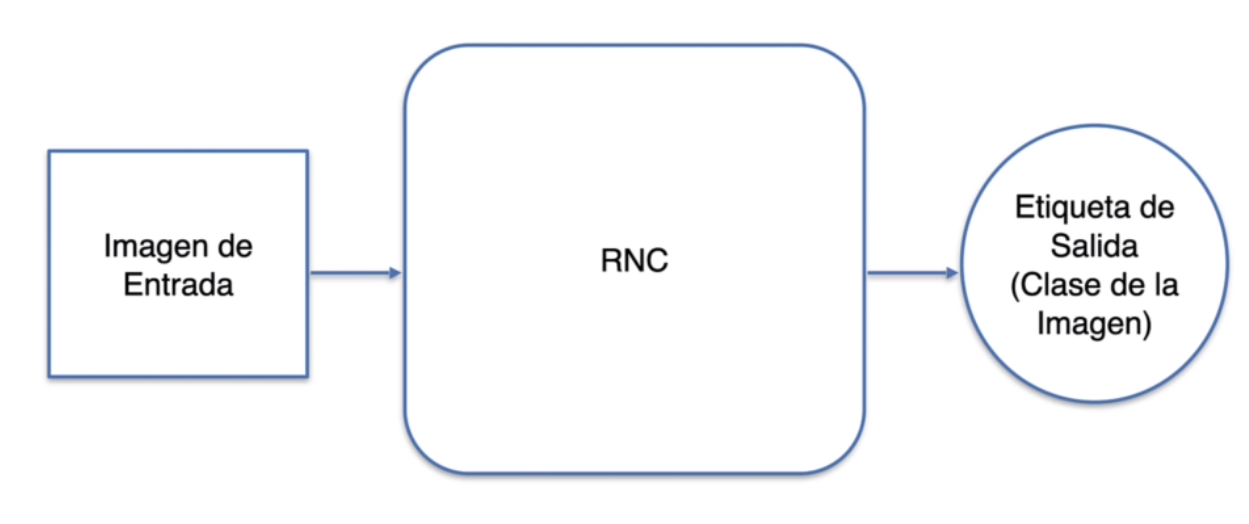
\includegraphics[width=0.8\textwidth]{img/Akwtp537HU.png}
        \end{figure}
\end{frame}

\begin{frame}
    Enfoque:\\
    \centering
        CNN (RNC) para NLP 
        \vspace{0.5cm}
        \begin{figure}
            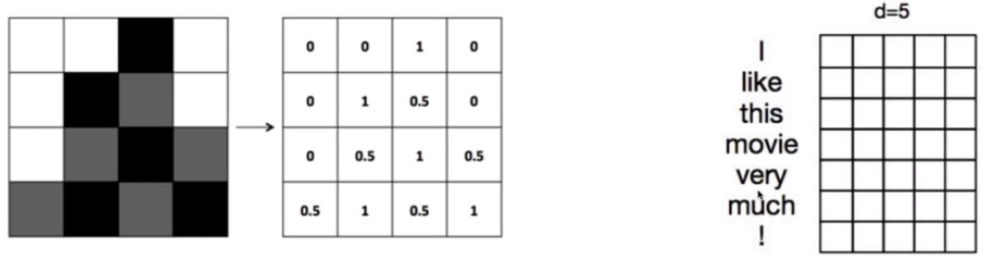
\includegraphics[width=0.8\textwidth]{img/rpyWSSZN22.png}
        \end{figure}
\end{frame}



\section{Corpus}
\begin{frame}
    \frametitle{Corpus}
    Se recolectará un dataset extrayendo tweets, y dada la temporada política que se esta llevando actualmente en el país hay una alta probabilidad de que estén fuertemente relacionados.

    \vspace{0.5cm} \pause

    Haciendo uso de las APIs \cite{api-tweet} de Twitter y python podrémos obtener un conjunto de tweets que contengan la relación de términos que buscamos/esperamos se presenten.


\end{frame}

\begin{frame}    
    \begin{itemize}
        \item \textbf{API Streaming}. Es utilizado para acceder, en tiempo real, a los tweets públicos
        \item \textbf{API Search}. Permite el acceso a los últimos 1500 tweets de los últimos 7 días.
        \item \textbf{API Rest}.Permite el acceso al núcleo de los datos de twitter y permite el acceso de los 3200 últimos tweets.
    \end{itemize}
\end{frame}



\section{Estrategias}
\begin{frame}
    \frametitle{Estrategias}    

    \begin{itemize}
        \item Obtención de los datos por medio de las herramientas de python para Twitter

        \item Realizar las estadísticas sobre los personajes políticos mas comentados.

        \item Eliminación de Tweets repetidos.
        
        \item Analizar el corpus en búsqueda de patrones de sentimientos y su comportamiento a través del tiempo.
    \end{itemize}
\end{frame}


\begin{frame}[allowframebreaks]
    \frametitle{References}
    \bibliographystyle{ieeetr}
    \bibliography{bib/biblio.bib}
\end{frame}


\end{document}